%% 
%% ACS project dissertation template. 
%% 
%% Currently designed for printing two-sided, but if you prefer to 
%% print single-sided just remove ",twoside,openright" from the 
%% \documentclass[] line below. 
%%
%%
%%   SMH, May 2010. 


\documentclass[a4paper,12pt,twoside,openright]{report}


%%
%% EDIT THE BELOW TO CUSTOMIZE
%%

\def\authorname{David Brazdil\xspace}
\def\authorcollege{Trinity Hall\xspace}
%\def\authoremail{Sarah.Jones@cl.cam.ac.uk}
\def\dissertationtitle{Java Native Interface on CHERI}
\def\wordcount{14,235}


\usepackage{epsfig,graphicx,parskip,setspace,tabularx,xspace,url,listings,color} 

%% START OF DOCUMENT
\begin{document}

\lstset{
	basicstyle=\tt\footnotesize,	% the size of the fonts that are used for the code
	numbers=left,			% where to put the line-numbers
	numberstyle=\footnotesize,	% the size of the fonts that are used for the line-numbers
	stepnumber=1,			% the step between two line-numbers. If it is 1 each line will be numbered
	numbersep=5pt,			% how far the line-numbers are from the code
	backgroundcolor=\color{white},	% choose the background color. You must add \usepackage{color}
	showspaces=false,		% show spaces adding particular underscores
	showstringspaces=false,		% underline spaces within strings
	showtabs=false,			% show tabs within strings adding particular underscores
	frame=leftline,			% adds a frame around the code
	tabsize=2,			% sets default tabsize to 2 spaces
	captionpos=b,			% sets the caption-position to bottom
	breaklines=true,		% sets automatic line breaking
	breakatwhitespace=false,	% sets if automatic breaks should only happen at whitespace
	escapeinside={\%*}{*)},		% if you want to add a comment within your code
	captionpos=t,			% title position
}

%% FRONTMATTER (TITLE PAGE, DECLARATION, ABSTRACT, ETC) 
\pagestyle{empty}
\singlespacing
% title page information
\begin{titlepage} 

\begin{center}
\noindent
\huge
\dissertationtitle \\
\vspace*{\stretch{1}}
\end{center}

\begin{center}
\noindent
\huge
\authorname \\
\Large
Computer Science Tripos, Part III \\
\authorcollege      \\[24pt]

\includegraphics{CUni3.eps}
\end{center}

\vspace{24pt} 

\begin{center}
\noindent
\large

\vspace*{\stretch{1}}
\end{center}

\begin{center}
\noindent
University of Cambridge \\
Computer Laboratory     \\
William Gates Building  \\
15 JJ Thomson Avenue    \\
Cambridge CB3 0FD       \\
{\sc United Kingdom}    \\
\end{center}

%\begin{center}
%\noindent
%Email: \authoremail \\
%\end{center}

\begin{center}
\noindent
\today
\end{center}

\end{titlepage} 

\newpage
\vspace*{\fill}

\onehalfspacing
\newpage
{\Huge \bf Declaration}

\vspace{24pt} 

I \authorname of \authorcollege, being a candidate for the M.Phil in
Advanced Computer Science, hereby declare that this report and the
work described in it are my own work, unaided except as may be
specified below, and that the report does not contain material that
has already been used to any substantial extent for a comparable
purpose.

\vspace{24pt}
Total word count: \wordcount

\vspace{60pt}
\textbf{Signed}: 

\vspace{12pt}
\textbf{Date}:


\vfill

This dissertation is copyright \copyright 2010 \authorname. 
\\
All trademarks used in this dissertation are hereby acknowledged.



\newpage
\vspace*{\fill}

\singlespacing
\newpage
{\Huge \bf Abstract}
\vspace{24pt} 

With the necessity to reuse legacy code, or to employ readily available third-party libraries, it is not uncommon for large applications to be written in more than one programming language. Such heterogeneous environments have inherent advantages, e.g.\ allowing security-critical components to be written in a memory-safe language like Java, while performance-critical code in C, but because there is no runtime separation between the two code bases, it is possible for the native code to corrupt the Java environment or to bypass its security.

Qishr demonstrates that the capability-enabled CHERI processor can be used to isolate Java native code into a safe sandbox, from which it can only interact with the Java runtime and the system kernel through a secure interface. It guarantees that the code cannot break memory safety of Java objects, controls its access to system resources in accordance with the security policy enforced by Java on its classes, and provides a compatibility layer for legacy code written against the standard native interface.

\newpage
\vspace*{\fill}


\pagenumbering{roman}
\setcounter{page}{0}
\pagestyle{plain}
\tableofcontents
\listoffigures
\listoftables

\onehalfspacing

%% START OF MAIN TEXT 

\chapter{Introduction}
\pagenumbering{arabic} 
\setcounter{page}{1} 

% This is the introduction where you should introduce your work.  In
% general the thing to aim for here is to describe a little bit of the
% context for your work --- why did you do it (motivation), what was the
% hoped-for outcome (aims) --- as well as trying to give a brief
% overview of what you actually did.
% 
% It's often useful to bring forward some ``highlights'' into 
% this chapter (e.g.\ some particularly compelling results, or 
% a particularly interesting finding). 
% 
% It's also traditional to give an outline of the rest of the
% document, although without care this can appear formulaic 
% and tedious. Your call. 



\begin{enumerate}
	\item Java applications need 
\end{enumerate}

\chapter{Background} 

% A more extensive coverage of what's required to understand your 
% work. In general you should assume the reader has a good undergraduate 
% degree in computer science, but is not necessarily an expert in 
% the particular area you've been working on. Hence this chapter 
% may need to summarize some ``text book'' material. 
% 
% This is not something you'd normally require in an academic paper, 
% and it may not be appropriate for your particular circumstances. 
% Indeed, in some cases it's possible to cover all of the ``background'' 
% material either in the introduction or at appropriate places in 
% the rest of the dissertation. 

\section{Java Security Architecture}

Java was designed mainly as a universal platform for networked environments which necessarily made its security model one of the most important architectural features. On all its levels, Java addresses the common pitfalls of modern software engineering which can lead to introduction of security vulnerabilities, and thus guarantees a minimal level of application robustness and alleviates the process of implementing additional security measures.

At the core of the platform lies the Java programming language, an easy-to-learn type-safe language with automatic memory management and built around the principles of object-oriented programming. These properties significantly reduce the likelihood of writing unsafe code and also encourage the principle of least privilege via separation of executable code and its state into smaller object-level protection domains.

Java applications are expected to be distributed over public networks and therefore the platform has to account for composition of code with varying level of trust. Untrusted code can be executed inside a safe environment isolated from other code running inside the same virtual machine and be subject to a programmatically managed security policy which can limit its access to guarded resources. This is called the \emph{Java Sandbox Model}.

Additionally, the Java framework provides a large set of extensible security APIs with ready-to-use implementation of many cryptographic algorithms and standardized protocols for public key infrastructure, authorization and encrypted network communication. 

\subsection{Code Safety}

The security of the Java platform is deeply rooted in the type, memory and control flow safety properties of its executable code. The language and the instruction set were crafted in a way that program bugs are likely to be caught by the compiler and pre-execution bytecode verifier, and other will raise an exception at runtime. 

% Java's type system is dynamic, although most types are actually checked statically for the sake of performance. Operations which are checked at runtime include array assignments, operations on generic classes and type casts. Unfortunately, the type inference algorithm has been shown to contain vulnerabilities~\cite{Suenaga:2012:JavaVulnerability} which make way to type confusion attacks~\cite{Oh:2012:JavaExploitReport} and these can subsequently be exploited to bypasss the security of the entire platform~\cite{McGraw:1999:SJG:298616}.

Memory safety in Java is strongly connected to the principles of OOP. Code does not have direct access to the heap but rather has to adhere to a model of a memory space structured into object instances and their internal fields protected by the reference monitor, accessed through opaque references and automatically managed by the garbage collector. Together with the type system and explicit range checks, Java prevents common bugs which can give the attacker access to an arbitrary part of the memory, such as buffer overflow or dangling pointers.

\subsection{Object Encapsulation}

The guarantees described above are the cornerstone of the Java security as they allow for isolation of individual software modules by enabling them to encapsulate their state. 

Individual classes therefore become separate protection domains which only permit the modification of their inner state through a set of transactions exposed in their public interface. These methods become the only entry points into the respective protection domain and can be used by the object to control access to its state and to prevent operations which could leave the state inconsistent.

Limiting the scope of the code which can access the state also makes it possible to argue about the high-level security properties of an object class. As the authors of Joe-E [REF] point out, however, Java still contains language features which can prevent such reasoning and suggest building a more secure platform around its safe subset.

\subsection{Java Sandbox Model}

The design of the Java platform was deeply influenced by the web and the ability to dynamically load executable code from various, potentially untrusted sources into one instance of the Java virtual machine a priority. The language safety properties do protect the integrity of the memory, but just by themselves cannot prevent the external code from abusing the system resources available to the VM or interacting with code from a different source. To this end, the platform provides a number of access control mechanisms which make it poosible to execute differents portions of the loaded code with different sets of permissions available to them. 

\begin{figure}
	\centering
	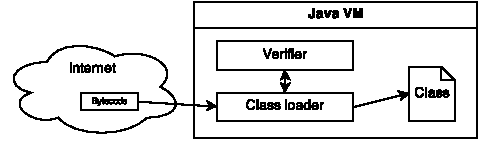
\includegraphics[width=0.8\textwidth]{dia_java_classload.pdf}
	\caption{Class loading in Java}
\end{figure}

Java code is loaded into the virtual machine by a special object which extends the \texttt{ClassLoader} class. The main task of a class loader is extracting bytecode from some external source and passing it on to the bytecode verifier which determines whether it complies with the required language safety properties. Typically it also selects the desired security policy which will be later enforced upon it, and it is the class loader's task to make sure that the newly loaded code will not replace any existing classes (including itself and other security-critical classes) unless this is explicitly allowed. 

Every Java VM provides a simple "primordial" class loader implemented in native code which bootstraps the framework and immediately hands the process over to its loader. Code with sufficient permissions can then define new, potentially simultaneosly active class loaders and arrange them into hierarchies. Since class loaders are also responsible for resolving classes and methods for the code loaded by them, they can be used to create local namespaces, effectively isolating codebases which should not be allowed to interact.

The last component of the Java sandbox is a reference monitor, called the Security Manager. Before untrusted code is called, the parent can set a thread-local reference to a \texttt{SecurityManager} object which implements the security policy that is to be enforced upon it. Should the untrusted code attempt to access system or VM resources during its execution, it must do so through the framework API and these methods always consult the active Security Manager before access is granted.

\subsection{Java Native Interface}

Just like bytecode, shared libraries are loaded by a class loader and reside in its namespace. The method resolver then uses a naming convention defined in the JNI specification to bind a class method which is marked \texttt{native} with a corresponding function in the native library.

\begin{figure}
	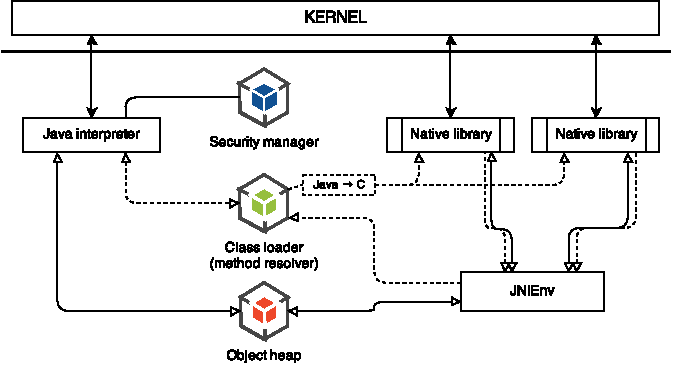
\includegraphics[width=\textwidth]{dia_jni_orig.pdf}
	\caption{Schematic diagram of the core JVM security components with respect to native code. Solid lines represent data flow paths, dashed lines show control flow.}
	\label{fig:OverviewJNI}
\end{figure}

\begin{figure}[t]
	\lstinputlisting[language=Java,title=HelloJNI.java]{example/HelloJNI.java}
	\lstinputlisting[language=C,title=HelloJNI.c]{example/HelloJNI.c}
	\caption{Example of a method implemented with JNI. \texttt{getMessage} calls \texttt{NewStringUTF} which instantiates a new \texttt{String} object and returns its reference to the caller.}
	\label{listing:HelloJNI}
\end{figure}

Developers are provided with a C/C++ header which contains the definitions of types compatible with the primitive types used in Java, the \texttt{jobject} type to represent object references (typically pointers to the object heap) and the \texttt{JNIEnv} data structure containing functions that provide an API for interfacing with the VM, such as reading/assigning values of object fields, creating new objects, or invoking other methods in the Java environment. A pointer to an instance of \texttt{JNIEnv} is passed to the function together with the actual parameters of the corresponding method call. Figure~\ref{fig:OverviewJNI} gives a simplified overview of the architecture, and Figure~\ref{listing:HelloJNI} shows an example of a simple Java class with a \texttt{native} method implemented in C.

However, the Java platform does not provide any means of containing native code. Because it resides in the same virtual address space as the VM, it does have unlimited access to the object heap and can both read and modify any object data on it, including the class loaders and other security-critical classes. Similarly, native code can perform system calls without the knowledge of the security monitor or even modify the state of the virtual machine.

What follows from this is that only applications which are written in pure Java can be sandboxed as any native code attached to the virtual machine can circumvent all of the security mechanisms it provides. Hence giving a piece of code the permission to load native libraries is equivalent to giving it all the other permissions as well as unlimited access to the state of the VM. This permission must therefore be taken away from all sandboxed code.

\subsection{Trust and Native Code}

Previous sections have explained the role of the three pillars of Java security: language safety, secure class loading and a reference monitor. To understand how native code fits into this picture, it is essential to understand the relationship between these three components and the assumptions they make.

The Java VM consists mainly of: bytecode interpreter (or a compiler into native code), a minimal class manager with a bytecode verifier, memory management code and a small set of low-level classes implemented in native code which faciliate communication between the VM and the managed code, e.g. to provide reflection. The entire VM codebase must be fully trusted and guarantee that only safe code will ever be executed.

The Java framework, on the other hand, is mostly written in Java with a relatively small number of native methods which give managed code access to system calls and only these therefore need to be trusted to not violate language safety. The framework includes classes which abstract over the system resources, provides its own class loader, which selects the appropriate security policy and passes bytecode over to the VM's verifier and loader, and a default implementation of the security manager. All of these Java classes, as well as the native code, are trusted to not compromise the class hierarchy and to always enforce the active security policy.

\section{Security with Capabilities}

Memory protection and decomposition of software into isolated components are highly desired security properties but contemporary computer systems do not provide the means of achieving them. Most commonly, operating systems provide controlled process isolation with virtual addressing and inter-process communication. This approach, however, suffers from poor scalability due to a high performance penalty imposed by the translation look-aside buffer as the number of protection domains and the domain switches between them increases. [better explain - why is it important here?] [REF] 

Conversly, capabilities have proven to be a security primitive which allows for fine-grained memory protection and low-overhead software compartmentalization within a single address space. This makes them an ideal tool for applying the principle of least privilege on a very small scale, i.e. running each software component with only the access rights it needs, and that in turn mitigates the consequences of security vulnerabilities which inevitably appear in the code. 

\subsection{CHERI}

Capability Hardware Enhanced RISC Instructions (CHERI) is an extension of the comodity 64-bit MIPS Instruction Set Architecture (ISA), developed at University of Cambridge Computer Laboratory, which adds capabilities as a new security primitive that can be utilized by the operating system and other software running on top of it. The result is a hybrid capability architecture which is backwards-compatible with the traditional form of process isolation with virtual address spaces, but simultaneously enables capability-aware software to employ additional security measures within the address space assigned to the running process.

% TODO: what it is you can do with CHERI (memory region, sealed, object, sandbox, ephemeral)

\subsection{Technical Details}

\chapter{Related Work} 

This chapter covers relevant (and typically, recent) research 
which you build upon (or improve upon). There are two complementary 
goals for this chapter: 
\begin{enumerate} 
  \item to show that you know and understand the state of the art; and 
  \item to put your work in context
\end{enumerate} 

Ideally you can tackle both together by providing a critique of
related work, and describing what is insufficient (and how you do
better!)

The related work chapter should usually come either near the front or
near the back of the dissertation. The advantage of the former is that
you get to build the argument for why your work is important before
presenting your solution(s) in later chapters; the advantage of the
latter is that don't have to forward reference to your solution too
much. The correct choice will depend on what you're writing up, and
your own personal preference.

\section{Joe-E}

\section{Dalvik}

sandbox by linux uid

\section{SafeJNI}

\section{Robusta}

doesn't support dynamic loading (and by design cannot)

\section{Capsicum}

\chapter{Design and Implementation} 

This chapter may be called something else\ldots but in general 
the idea is that you have one (or a few) ``meat'' chapters which
describe the work you did in technical detail. 

\section{Overview}

\subsection{Toolchain}

\section{Sandboxing}

\subsection{Security domains}

\section{Enforcing memory safety}

\section{Applying security policy}

all Java domains - language safety, security policies

VM domain remains the only one that can do system calls => GNU Classpath now provides services around system calls but those must go through the trusted trampoline

\section{Garbage collection}

\chapter{Evaluation} 

For any practical projects, you should almost certainly have
some kind of evaluation, and it's often useful to separate 
this out into its own chapter. 


\chapter{Summary and Conclusions} 

As you might imagine: summarizes the dissertation, and draws 
any conclusions. Depending on the length of your work, and 
how well you write, you may not need a summary here. 

You will generally want to draw some conclusions, and point
to potential future work. 




\appendix
\singlespacing

\bibliographystyle{unsrt} 
\bibliography{acs-dissertation} 

\end{document}
